% !TeX root = ..\studio-operation-guide.tex
\section{Answering Calls}

When you are not in another call, you can answer a call in one of three ways:

\begin{itemize}
	\item Using the handset
	\item Using the speakerphone
	\item Using the headset
\end{itemize}

\begin{quote}
	\textbf{Note}
	
	You can reject incoming calls by pressing the \textbf{X} key, or the
	\textbf{Reject} soft key. You can also activate Do Not Disturb mode to
	reject all incoming calls without ringing on your phone. For more information,
	refer to Do Not Disturb (DND) on page 84.

	You can forward incoming calls to someone else by pressing the
	\textbf{Forward} soft key. For more information, refer to Call Forward on
	page 88.
\end{quote}

\subsection{Answering When Not in Another Call}

Call duration and destination will always appear on the LCD screen for
the active call.

\subsubsection{To answer a call using the handset:}

\begin{enumerate}
	\item Pick up the handset.
\end{enumerate}

\subsubsection{To answer a call using the hands-free speakerphone mode:}

Do one of the following:

\begin{itemize}
	\item Press \scalerel*{
\includegraphics{images/yealink/btn-speaker.png}}{B}.
	\item With the handset on-hook and the headset mode deactivated, press the
		\textbf{Answer} soft key.
	\item With the handset on-hook and the headset mode deactivated, press the
		line key (the line key LED flashes green).
\end{itemize}

\subsubsection{To answer a call using the headset:}

Do one of the following:

\begin{itemize}
	\item Press \scalerel*{
\includegraphics{images/yealink/btn-headset.png}}{B}.
	\item With the headset mode activated, press the \textbf{Answer} soft key.
	\item With the headset mode activated, press the line key (the line key LED
		flashes green).
\end{itemize}

\subsection{Answering When in Another Call}

If you have an active call, and an incoming call arrives on the phone,
do one of the following:

\begin{figure}[h]
	\centering
	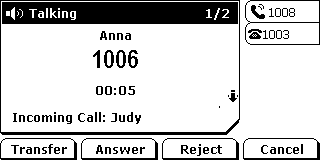
\includegraphics{images/yealink/screen-002.png}
\end{figure}

\begin{itemize}
	\item Press the \textbf{Answer} soft key.

		The incoming call is answered and the original call is placed on hold.
	\item Press \scalerel*{
\includegraphics{images/yealink/btn-up.png}}{B} to
		access the new call.

		\begin{figure}[h]
			\centering
			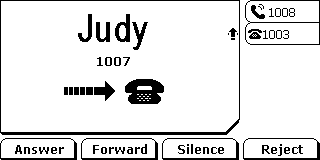
\includegraphics{images/yealink/screen-003.png}
		\end{figure}

		Press \scalerel*{
\includegraphics{images/yealink/btn-ok.png}}{B} or
		the \textbf{Answer} soft key.

		The incoming call is answered and the original call is placed on hold.
\end{itemize}
